%==========================================================================
%Template File for Monthly Lectual Meeting
%2006/05/22 (kkobayashi@mikilab.doshisha.ac.jp)
%==========================================================================
\documentclass[a4j,9pt,twocolumn]{jsarticle}
\usepackage{mlm2.0}
\usepackage{epsf}
\pagestyle{plain}
\usepackage{url}
\usepackage{subfigure}
\setcounter{page}{1}
\usepackage{geometry}
\geometry{left=25mm,right=25mm,top=20mm,bottom=30mm}
%\usepackage[dvips]{graphicx}

\begin{document}
\twocolumn[
%---------------------------------------------------------------------------        % ヘッダ    書式:\beginheader{回}{年}{月}
%---------------------------------------------------------------------------
\beginheader{171}{2016}{04}
%---------------------------------------------------------------------------
% 発表題目    書式:\title{日本語}{英語} 「\\」で改行できます
%---------------------------------------------------------------------------
\title%
{git}%
%{更なる大容量化を目指して 進化しつづける次世代光メディア}

%---------------------------------------------------------------------------
% 著者名      書式:\author{日本語著者名}{英語著者名}
%---------------------------------------------------------------------------
\author{山下 俊樹,外村 篤紀\\Toshiki YAMASHITA,Atsuki TONOMURA}

%---------------------------------------------------------------------------
\endheader
%\begin{abstract}
%---------------------------------------------------------------------------
%Recently, a DVD attracts attention along with the image and the digitization of the sound. The standards of these DVD are complicated. So, in this paper, the standards of the DVD are summarized and the DVD of the next generation is refered. 
%---------------------------------------------------------------------------
%\end{abstract}
]

%---------------------------------------------------------------------------
% 本文
%---------------------------------------------------------------------------

\section{はじめに}
近年,ソフトウェアの大規模化にともない,プログラムの更新頻度は増加傾向にある.そこで,コンピュータ上で作成または編集したファイルの変更履歴を管理するバージョン管理システムは,より重要となっている.本稿では,バージョン管理システムの1つであるgit,および関連サービスのGitHubについて述べる.

\section{git}
\subsection{概要}
gitはバージョン管理システムの1つである.バージョン管理システムには,管理下のファイルを任意の記録時点の状態に復元できることや,1つのファイルを複数人で編集する場合,競合が発生しないように管理が行えることなどの利点がある\cite{pop}.gitで管理されるファイルやディレクトリの変更内容は,リポジトリと呼ばれるデータベースに蓄積される.

\subsection{構成}
gitの構成を\fgref{git}に示す.

\begin{figure}[h]
\centering
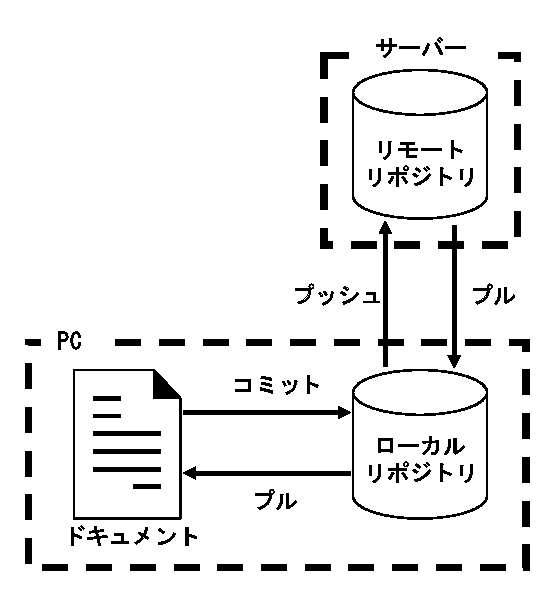
\includegraphics[width=80mm]{img/git.eps}
\caption{gitの構成}
\label{git}
\end{figure}

分散型バージョン管理システムにおけるリポジトリは2種類に大別できる.1つは,サーバ上に配置され複数ユーザで利用するリモートリポジトリである.もう1つは,個人のPC内に配置され,その個人が利用するローカルリポジトリである.ファイルやディレクトリの変更をローカルリポジトリに記録する操作をコミットと呼ぶ.コミットやプッシュを行うことで作業成果を記録する.また,プルを行うことでリモートリポジトリから他者の作業成果をダウンロードして統合する.

ローカルリポジトリによって,ネットワークに接続されていない環境でもコミットを行うことができる.あるいは,バグ修正のために個人のローカルリポジトリに適量のコミットを行い,修正を完了したとする.その後,修正が完了したソフトウェアをリモートリポジトリにプッシュし,他者に公開する方法が可能である.

\begin{figure}[h]
\centering
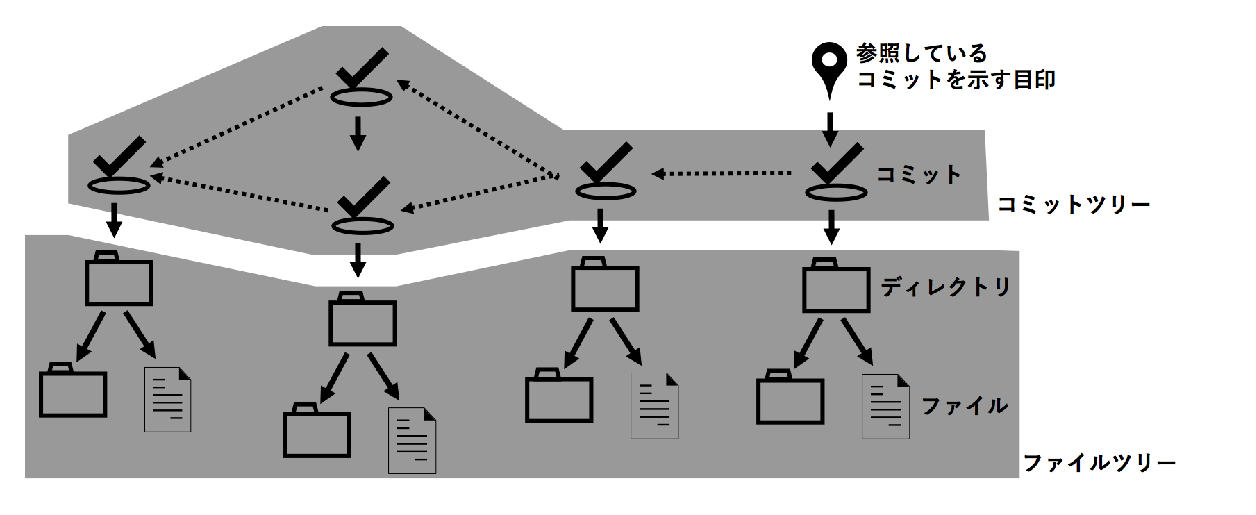
\includegraphics[width=90mm]{img/tree2.eps}
\caption{ツリー構造}
\label{tree}
\end{figure}

次に,バージョン管理手法について述べる.コミットを行うと,対象のディレクトリの内容がリポジトリに全て保存される.参照しているコミットには目印が付けられており,目印からコミットを辿ることで,いかなるコミットの対象ファイルやディレクトリにも芋づる式にアクセスできる.

コミットの時系列順の管理は,コミットツリーで行う.コミットツリーとは,コミット間のポインタで繋がれたツリー構造である.1つのコミットで管理される複数のファイルやディレクトリは,ファイルツリーと呼ばれるツリー構造で表される.したがって,任意のコミット時点の状態に戻す場合は,目印からコミットツリーをたどり,対応するファイルを取り出せばよい.gitの動作は目印による管理のために,高速である.

\subsection{ブランチ}
gitの特徴の1つであるブランチは,蓄積されたコミットの時系列を指す.すなわち,複数回のコミットを作成順に並べた連なりをブランチと呼ぶ.また,ブランチを分岐する操作もブランチと呼ぶ.分岐したブランチ同士は互いに独立しており,異なる内容の更新を同時に行える.ブランチ同士の結合はマージと呼ぶ.ブランチを利用した例を\fgref{branch_ex}に示す.

\begin{figure}[h]
\centering
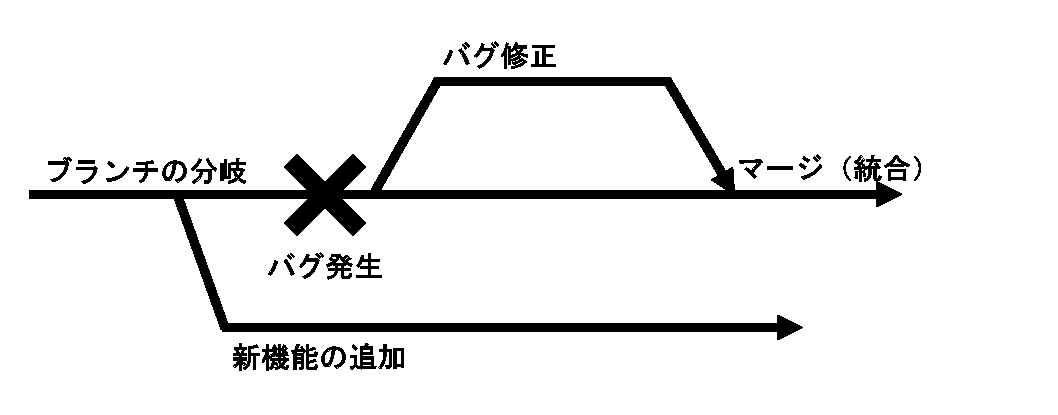
\includegraphics[width=80mm]{img/branch.eps}
\caption{ブランチの例}
\label{branch_ex}
\end{figure}

ブランチを用いることで,様々な開発やバグ修正などを並行して行うことができる.\fgref{branch_ex}において既に運用されているソフトウェアの管理を行っているブランチをmasterブランチとし,そのソフトウェアのバグを修正するために用意したブランチをbugfixブランチとする.この場合,二つのブランチは独立しているため,masterブランチに影響を与えることなくbugfixブランチでバグ修正を行うことができる.すなわち,ブランチを用いない場合は,バグ修正が完了するまでソフトウェアの運用を停止しなければならない.それに対し,ブランチを用いれば,ソフトウェアの運用を止めることなく,平行してバグ修正を行うことができる.バグ修正が完了した後にマージを行った時点でバグが修正される.さらに,ブランチの本数を増やせば,リリースしたソフトウェアを運用しながら新機能の追加を行い,加えてバグ修正も同時に行うといった運用が可能である.

gitのブランチは,他のバージョン管理システムに比べて優れている.他のシステムでは,マージの際にどのファイルをどのようにマージするか明示的に入力する必要があるが,gitは自動的に行うことができる.また,マージにかかる時間も他のシステムに比べて高速である.

\section{GitHub}
\subsection{概要}

\begin{figure}[h]
\centering
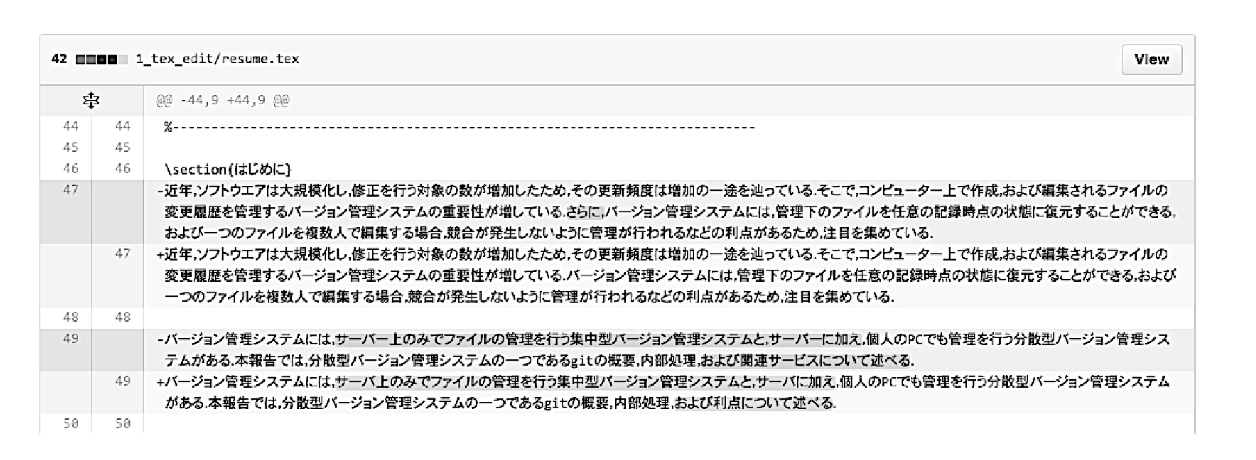
\includegraphics[width=85mm]{img/github.eps}
\caption{GitHubのGUIの例}
\label{github}
\end{figure}

GitHubとは,gitを利用したSNSである.現在,Githubは最も人気のあるgitサービス提供サイトであり,そのユーザ数は1000万人を超えている\cite{github}.GitHubの特徴の1つは,分かりやすいGUIである.\fgref{github}に,前回のコミットからの変更点が,色分けにより分かりやすく示されている例を示した.また,GitHubのユーザはリモートリポジトリを無料で持つことができるため,他のユーザと協力してソースコードを管理できるサービスとして広まった.他のユーザと協力するための機能として,コードレビュー,コメント機能などがある.コードレビューとは,ソースコードに含まれる誤りを検出,修正することを目的として行われるソースコードの査読を指す.これらの機能を用いることで,ユーザのソースコードが他者の目に触れ,コメントが付く.その結果,ユーザによる修正が行われ,ソースコードのバグが解消や可読性の向上などの利点を生む.

\subsection{機能}
フォーク機能について述べる.GitHubにおけるフォークはブランチの分岐操作を指す.フォークによって,ユーザが他のユーザのリポジトリからフォークしたブランチを用いて開発を行うことができる.利点は,ソフトウエアのデバッグを開発者以外のユーザが行えることである.さらに,初心者がある程度完成されたソフトウエアをフォークすれば,フォーク元の本体には影響を与えず,様々な改変を行いながら学習ができることなどが挙げられる.

次に,チケット機能について述べる.GitHub内ではIssueと呼ばれているが,本稿ではチケットと同義とする.チケットとは,作業をタスクに分割し,タスク1つ1つに対して割り振られるものである.開発者は発行されたチケットを取り,それに記されたタスク(バグ修正など)をこなし,タスクが完了するとコミットを行い,チケットを消去(クローズ)する.この一連の流れでタスクを管理する.タスクをチケットで管理することにより,作業の全容が把握しやすいことや,チームでの開発においてタスクの分配が行い易くなることなどの利点がある.また,チケットを用いて行うチケット駆動開発は,アジャイル開発とも親和性が高いため,注目を集めている.チケット駆動開発を行う際には,オンラインプロジェクト管理ソフトウェアであるRedmineなどを併用する場合が多い.

GitHubの利点は上記の通りである.一方,欠点としてGitHubで作成したリモートリポジトリは全て公開されるため,ソースコードを公開しない場合の多いWebデザインなどのソースコード管理には不具合が発生する.また,GitHubは外部サービスであるため,サーバ障害などが発生した場合に関連サービスが使用不能になる危険性がある.実際に,2016年1月28日にサービス障害が発生し,多くのユーザや企業が被害を被った\cite{news}.

\subsection{関連サービス}
GitHubに競合するサービスとして,BitBucketが挙げられる. Githubに対して,非公開のリモートリポジトリを作成できる,及びgit以外の分散型バージョン管理システムであるMercurialを使用できるなどの利点がある.どちらのサービスもソーシャルコーディングの普及に貢献していると言えるが,現時点でのユーザ数はGitHubが圧倒的に多い.これは,GitHubに対応する周辺サービスが多いことや,GUIが使いやすいことなどによる.

\section{今後の展望}
今日,ソフトウェアのリリース速度は増加の一途を辿っている.それにともない,開発の効率化,高速化が重要視されている.そのため,gitのようなバージョン管理ソフトウェアは更に普及すると考えられる.また,GitHubのようなgitを用いたサービスは,現在概ね無料で公開されているが,あるソフトウェアの開発において,デバッグや開発の一部を他者に依頼し,一番良いソースコードを含むフォークに報酬を払うなどのビジネスも近い将来に生まれると考える.

\small
\begin{thebibliography}{99}
\bibitem{pop}
岡本隆史:Gitに潜む光と闇,入手先,(http://gihyo.jp/dev/column/01/prog/2012/git)

\bibitem{mecha}
koseki2:Git の仕組み (1),入手先(http://koseki.\\hatenablog.com/entry/2014/04/22/inside-git-1)

\bibitem{github}
Ken Nishimura,市民生活をオープンデータ活用で改善する政府や地域行政の事例 [GitHub Universe],(http://thebridge.jp/2015/10/github-universe-session-changing-lives-with-open-data).

\bibitem{news}
Yukari Mitsuhashi,GitHub、1月末のダウンの原因はデータセンターでの停電と説明,(http://www.itmedia.co.jp/news/articles/1602/\\01/news070.html).
\end{thebibliography}
\end{document}